\documentclass[12pt,twoside]{article}
\usepackage[UTF8]{ctex}             %确保中文可正常显示的包
\usepackage{amsmath}                %确保公式可正常显示的包
\usepackage{multicol}               %分栏操作的包
\usepackage{ragged2e}               %文本对齐操作的包
\usepackage{geometry}               %设置纸张属性的包
\usepackage{graphicx}               %插入图片的包
\usepackage{float}                  %让图片浮动
\usepackage{fancyhdr}               %页眉页脚
\setlength{\columnsep}{7mm}         %设置栏间距
\numberwithin{equation}{section}    %公式按照章节编号
\geometry{left=2cm,right=2cm,top=2cm,bottom=2cm}

%设置页眉页脚
\pagestyle{fancy}
\fancyhf{}
\lhead{西南大学}
\fancyhead[OC]{理论力学课程论文}
\fancyhead[EC]{Course Paper on Theoretical Mechanics}
\rhead{本科生课程论文}

\lfoot{}
\cfoot{\thepage}
\rfoot{}
%设置页眉页脚

\begin{document}

\thispagestyle{empty}
\pagenumbering{gobble}              %临时关闭页码计数

%封面部分

\begin{figure}[H]
    \centering
    
\includegraphics{img/fengmian.png}
\end{figure}

\vspace{-2cm}   
\hspace{12.75cm} 
\begin{tabular}{|c|}
    \hline
    成绩： \\
    \hline
    \\
    \hline
\end{tabular}

\vspace{1\baselineskip}             %空行
\begin{center}
    \heiti\fontsize{36}{30}
    本科生课程论文
\end{center}

\vspace{2\baselineskip} 

\begin{center}
    
    \heiti\fontsize{16}{24}\selectfont
    论文题目:\underline{\makebox[10cm]{\songti{变质量拉格朗日方程}}}
    
    \heiti\fontsize{16}{24}\selectfont
    课程名称:\underline{\makebox[10cm]{\songti{理论力学}}}

    \heiti\fontsize{16}{24}\selectfont
    任课教师:\underline{\makebox[10cm]{\songti{xxx}}}

    \heiti\fontsize{16}{24}\selectfont
    专\hspace{2em}业:\underline{\makebox[10cm]{\songti{物理学}}}

    \heiti\fontsize{16}{24}\selectfont
    班\hspace{2em}级:\underline{\makebox[10cm]{\songti{x x级物理1班}}}

    \heiti\fontsize{16}{24}\selectfont
    学\hspace{2em}号:\underline{\makebox[10cm]{\songti{xxxxxx}}}

    \heiti\fontsize{16}{24}\selectfont
    姓\hspace{2em}名:\underline{\makebox[10cm]{\songti{xx}}}
    
\end{center}

\vspace{\baselineskip} 

\begin{center}
    \framebox[12.5cm]{
    \parbox[t][5cm][t]{12.5cm}{
    \hspace*{10pt}教师评语：
    }
    }
\end{center}

\begin{center}
    2024年12月11日
\end{center}

%封面部分


\newpage
\pagenumbering{arabic}              %重新开启阿拉伯数字页码
\setcounter{page}{1}                %将页码计数器重置为1
\begin{center}
    \heiti\zihao{1}
    变质量拉格朗日方程                %标题
\end{center}

%\tableofcontents                   %设置目录
%\newpage                           %另外起一页

\begin{center}
    Peng Yu                         %作者及单位

    (西南大学，物理科学与技术学院，2023级，物理1班)
\end{center}

\begin{flushleft}                   %文本左对齐（用于取消自动首行缩进）
    \justifying                     %两端对齐
    \textbf{摘 \hspace{0.5em} 要：}拉格朗日方程在分析力学中扮演着极为重要的角色，它从能量的角度出发，给出了一条寻找复杂系统运动微分方程方便快捷的道路。但在书写系统的拉格朗日方程时，要求所研究的系统是恒质量系统，因此在使用拉格朗日方程处理变质量系统的动力学问题时，还需要对其进行拓展，需添加一项因为质量变化而产生的附加广义力。本文将利用数学分析从牛顿第二定律和虚功原理出发给出变质量系统对应拉格朗日方程的详细推导过程，并利用导出的变质量拉格朗日方程研究经典情形与狭义相对论情形下的变质量问题。\\
    \textbf{关键词：}变质量；拉格朗日方程；附加广义力；狭义相对论
\end{flushleft}

\begin{multicols}{2}                %创建双栏

    \section{引言}
    随着经典力学和数学分析的不断发展，1788年拉格朗日出版了最早的分析力学著作《分析力学》，他利用严谨且优雅的数学，以虚功原理和达朗贝尔原理为基石得到动力学的普遍方程——拉格朗日方程，几乎所有的分析力学的动力学方程都是从这个方程直接或间接导出的.\cite{zhou2001}下面我们将利用数学分析，从牛顿第二定律出发，得到含质量导数达朗贝尔——拉格朗日原理，以此推导出理想约束下变质量系统中的拉格朗日方程，并给出保守系统中含拉格朗日量的变质量拉格朗日方程，最后基于所得到的理论处理经典力学中的变质量问题并讨论狭义相对论情形下的变质量问题\cite{yang1989}.

    \section{变质量的拉格朗日方程}
    \subsection{含质量导数的达朗贝尔——拉格朗日原理}
    设有一个含$N$个质点的变质量系统，研究第$i$个质点，$t$时刻的质量为$m_i$，速度为$\vec{v}_i$，在$t+\Delta t$时刻，发生$\Delta m_i$的质量输运，输运速度为$\vec{u}_i$，其质量变为$m_i+\Delta m_i$速度变为$\vec{v}_i+\Delta \vec{v}_i$，那么由动量定理有
    \begin{equation}
        \begin{split}
            (m_i+\Delta m_i)(\vec{v}_i+\Delta\vec{v}_i) - \\ m_i\vec{v}_i - \Delta m_i\vec{u}_i = \vec{F}_i\Delta t
        \end{split}
        \label{eq:1}
    \end{equation}
    其中$\vec{F}_i$为发生质量输运时的相互作用，略去高阶小量上式变为
    \[
    \Delta m_i\vec{v}_i+m_i\Delta \vec{v}_i-\Delta m_i\vec{u}_i=\vec{F}_i\Delta t
    \]
    将其写为微分形式为
    \begin{equation}
        \frac{d\left( m_i\vec{v}_i \right)}{dt}-\vec{u}_i\frac{dm_i}{dt}=\vec{F}_i
        \label{eq:2}
    \end{equation}
    \eqref{eq:2}式便是经典牛顿力学中处理变质量问题的重要公式.将输运质量的速度$\vec{u}_i$写为相对第$i$个质点的速度$\vec{v}_{ri}$与第$i$个质点速度$\vec{v}_i$的和易得

    \begin{equation}
        m_i\frac{d\vec{v}_i}{dt} = \vec{F}_i + \vec{v}_{r_i} \frac{dm_i}{dt}
        \label{eq:3}
    \end{equation}

    分析\eqref{eq:3}可知式可以知道，在该变质量系统中，第$i$个质点所受的合外力除发生质量输运间的相互作用外，还有因质量变化而引起的作用力，这部分作用力的大小为输运质量的相对速度与质量变化率的乘积.因此，利用分析力学处理变质量问题时，还需引入因质量变化而引起的作用力，设该作用力为$\vec{\beta}_i$，那么$\vec{\beta}_i=\vec{v}_{ir}\dot{m}$.则由牛顿第二定律有
    \begin{equation}
        \vec{F}_i+\vec{R}_i+\vec{\beta}_i=m_i\ddot{\vec{r}}_i
        \label{eq:4}
    \end{equation}
    由虚功原理有
    \begin{equation}
        \sum_{i=1}^N{\left( \vec{F}_i+\vec{R}_i+\vec{\beta}_i-m_i\ddot{\vec{r}}_i \right) \cdot \delta \vec{r}_i}=0
        \label{eq:5}
    \end{equation}
    上式中$\vec{R}_i$为引入的约束反力，$\delta r_i$为虚位移，若研究的是理想约束，那么
    \[
    \sum_{i=1}^N{\vec{R}_i\cdot \delta \vec{r}_i}=0
    \]
    则\eqref{eq:5}变为
    \begin{equation}
        \sum_{i=1}^N{\left( \vec{F}_i+\vec{\beta}_i-m_i\ddot{\vec{r}}_i \right) \cdot \delta \vec{r}_i}=0
        \label{eq:6}
    \end{equation}
    这便是含质量导数的达朗贝尔——拉格朗日原理
    \subsection{变质量的拉格朗日方程}
    考虑到$\vec{r}_i=\vec{r}_i\left( q_1,q_2,q_3,...,q_s;t \right) $，$q_{\alpha}$为广义坐标，那么
    \[
    \delta \vec{r}_i=\sum_{\alpha =1}^s{\frac{\partial \vec{r}_i}{\partial q_{\alpha}}}\delta q_{\alpha}
    \]
    将上式代入\eqref{eq:6}式中有
    \[
    \sum_{i=1}^N{\left( \vec{F}_i+\vec{\beta}_i-m_i\ddot{\vec{r}}_i \right) \cdot}\sum_{\alpha =1}^s{\frac{\partial \vec{r}_i}{\partial q_{\alpha}}}\delta q_{\alpha}=0
    \]
    交换求和顺序有
    \begin{equation}
        \sum_{\alpha =1}^s{\sum_{i=1}^N{\left( \vec{F}_i+\vec{\beta}_i-m_i\ddot{\vec{r}}_i \right) \cdot}\frac{\partial \vec{r}_i}{\partial q_{\alpha}}\delta q_{\alpha}}=0
        \label{eq:7}
    \end{equation}
    令$P_{\alpha}=\sum_{i=1}^N{m_i\ddot{\vec{r}}_i\cdot \frac{\partial \vec{r}_i}{\partial q_{\alpha}}}$，现计算$P_{\alpha}$
    \[
    \begin{split}
        P_{\alpha} &= \sum_{i=1}^N m_i \frac{d\dot{\vec{r}}_i}{dt} \cdot \frac{\partial \vec{r}_i}{\partial q_{\alpha}} \\
               &= \sum_{i=1}^N m_i \left[ \frac{d}{dt} \left( \dot{\vec{r}}_i \cdot \frac{\partial \vec{r}_i}{\partial q_{\alpha}} \right) - \dot{\vec{r}}_i \cdot \frac{d}{dt} \frac{\partial \vec{r}_i}{\partial q_{\alpha}} \right]
    \end{split}
    \]
    由于
    \begin{equation}
        \frac{\partial \vec{r}_i}{\partial q_{\alpha}}=\frac{\partial \dot{\vec{r}}_i}{\partial \dot{q}_{\alpha}}
        \label{eq:8}
    \end{equation}
    \begin{equation}
        \frac{d}{dt}\frac{\partial \vec{r}_i}{\partial q_{\alpha}}=\frac{\partial \dot{\vec{r}}_i}{\partial q_{\alpha}}
        \label{eq:9}
    \end{equation}
    那么$P_{\alpha}$可进一步化简为
    \begin{equation}
        P_{\alpha}=\sum_{i=1}^N{m_i\left[ \frac{d}{dt}\left( \frac{1}{2}\frac{\partial \dot{\vec{r}}_{i}^{2}}{\partial \dot{q}_{\alpha}} \right) -\frac{1}{2}\frac{\partial \dot{\vec{r}}_{i}^{2}}{\partial q_{\alpha}} \right]}
        \label{eq:10}
    \end{equation}
    考虑到$m_i$是广义坐标$q_{\alpha}$，广义速度$\dot{q}_{\alpha}$和时间的函数，即$m_i=m_i\left( q_{\alpha},\dot{q}_{\alpha};t \right) $，将$m_i$凑到微分中有
    \[
        \begin{split}
            P_{\alpha} &= \sum_{i=1}^N \left[ \frac{1}{2}\frac{d}{dt}\frac{\partial (m_i\dot{\vec{r}}_i^2)}{\partial \dot{q}_{\alpha}}
            - \frac{1}{2}\frac{d}{dt}\left( \frac{\partial m_i}{\partial \dot{q}_{\alpha}}\dot{\vec{r}}_i^2 \right) \right. 
            \\
            & \left. -\, \dot{m}_i\dot{\vec{r}}_i\cdot \frac{\partial \dot{\vec{r}}_i}{\partial \dot{q}_{\alpha}}- \frac{1}{2}\frac{\partial (m_i\dot{\vec{r}}_i^2)}{\partial q_{\alpha}}+ \frac{1}{2}\frac{\partial m_i}{\partial q_{\alpha}}\dot{\vec{r}}_i^2 \right]
        \end{split}
    \]
    令$T_i=\frac{1}{2}m_i\dot{\vec{r}}_{i}^{2}$，那么
    \[
        \begin{split}
            P_{\alpha} &= \sum_{i=1}^N{\left[ \frac{d}{dt}\frac{\partial T_i}{\partial \dot{q}_{\alpha}}-\frac{\partial T_i}{\partial q_{\alpha}}-\frac{1}{2}\frac{d}{dt}\left( \frac{\partial m_i}{\partial \dot{q}_{\alpha}}\dot{\vec{r}}_{i}^{2} \right) \right.}
            \\
            & \left. -\dot{m}_i\dot{\vec{r}}_i\cdot \frac{\partial \dot{\vec{r}}_i}{\partial \dot{q}_{\alpha}}+\frac{1}{2}\frac{\partial m_i}{\partial q_{\alpha}}\dot{\vec{r}}_{i}^{2} \right] 
        \end{split}
    \]
    将上式代入\eqref{eq:7}有
    \begin{equation}
        \frac{d}{dt}\left( \frac{\partial T}{\partial \dot{q}_{\alpha}} \right) -\frac{\partial T}{\partial q_{\alpha}}=Q_{\alpha}+\varPhi _{\alpha}
        \label{eq:11}
    \end{equation}
    上式中
    \[
        Q_{\alpha}=\sum_{i=1}^N{\vec{F}_i\cdot \frac{\partial \vec{r}_i}{\partial q_{\alpha}}}
    \]
    \[
        \begin{split}
            \varPhi_{\alpha} &= \sum_{i=1}^N \left[ \frac{1}{2}\frac{d}{dt}\left( \frac{\partial m_i}{\partial \dot{q}_{\alpha}}\dot{\vec{r}}_{i}^{2} \right) + \vec{u}_i\dot{m}_i\cdot \frac{\partial \vec{r}_i}{\partial q_{\alpha}} \right. 
            \\
            & \left. - \frac{1}{2}\frac{\partial m_i}{\partial q_{\alpha}}\dot{\vec{r}}_{i}^{2} \right]
        \end{split}
    \]
    其中$\vec{u}_i=\vec{v}_{ri}+\dot{\vec{r}}_i$，\eqref{eq:11}便是在变质量系统中的拉格朗日方程，$Q_{\alpha}$被称为广义力，$\varPhi _{\alpha}$是因系统质量变化而产生的附加广义力，实际上，\eqref{eq:11}与\eqref{eq:3}式形式上是统一的，均有一项因质量变化而产生的附加作用.可以发现，$\varPhi _{\alpha}$由质量因广义坐标$q_{\alpha}$变化，因时间$t$变化和因广义速度$\dot{q}_{\alpha}$变化产生的附加因子组成，但因广义速度变化产生的附加因子对$\varPhi _{\alpha}$贡献还要复杂一些.在实际问题的研究中，大多问题中的质量$m_i$仅为时间$t$的函数或仅为广义坐标$q_{\alpha}$的函数，下面讨论$m_i$的不同情况.

    当$m_i$仅是广义坐标$q_{\alpha}$的函数时，$m_i=m_i\left( q_{\alpha} \right) $，附加广义力的坐标分量为
    \begin{equation}
        \varPhi _{\alpha q}=-\frac{1}{2}\sum_{i=1}^N{\frac{\partial m_i}{\partial q_{\alpha}}\dot{\vec{r}}_{i}^{2}}
        \label{eq:12}
    \end{equation}
    当$m_i$仅是时间$t$的函数时，$m_i=m_i\left( t \right) $，附加广义力的时间分量为
    \begin{equation}
        \varPhi _{\alpha t}=\sum_{i=1}^N{\dot{m}_i\vec{u}\cdot \frac{\partial \vec{r}_i}{\partial q_{\alpha}}}
        \label{eq:13}
    \end{equation}
    当$m_i$仅是时间$\dot{q}_{\alpha}$的函数时，$m_i=m_i\left( \dot{q}_{\alpha} \right) $，附加广义力的速度分量为
    \begin{equation}
        \varPhi _{\alpha \dot{q}}=\frac{1}{2}\sum_{i=1}^N{\frac{d}{dt}\left( \frac{\partial m_i}{\partial \dot{q}_{\alpha}}\dot{\vec{r}}_{i}^{2} \right)}
        \label{eq:14}
    \end{equation}
    在其它情况下，$\varPhi _{\alpha}$则为$\varPhi _{\alpha q}$、$\varPhi _{\alpha t}$和$\varPhi _{\alpha \dot{q}}$的组合.

    \section{保守系统下的变质量拉格朗日方程}
    若$\vec{F}\left( \vec{r} \right) $为保守力场，那么其旋度为0，即
    \begin{equation}
        \nabla \times \vec{F}\left( \vec{r} \right) =0
        \label{eq:15}
    \end{equation}
    由矢量分析可知，该保守力场必定对应某个势函数$V$，并且此保守力场可以写为
    \begin{equation}
        \vec{F}\left( \vec{r} \right) =-\nabla V
        \label{eq:16}
    \end{equation}
    这样，广义力$Q_{\alpha}$便可以写为
    \[
        Q_{\alpha}=-\sum_{i=1}^N{\left( \frac{\partial \vec{r}_i}{\partial q_{\alpha}} \right) \cdot \nabla V}
    \]  
    对上式化简有
    \begin{equation}
        Q_{\alpha}=-\sum_{i=1}^N{\frac{\partial V_i}{\partial q_{\alpha}}}
        \label{eq:17}
    \end{equation}
    将上式代入\eqref{eq:11}有
    \[
        \frac{d}{dt}\left( \frac{\partial T}{\partial \dot{q}_{\alpha}} \right) -\frac{\partial \left( T-V \right)}{\partial q_{\alpha}}=\varPhi _{\alpha}
    \]
    定义拉格朗日函数$L=T-V$，将其代入上式中便得
    \[
        \frac{d}{dt}\left( \frac{\partial L}{\partial \dot{q}_{\alpha}} \right) -\frac{\partial L}{\partial q_{\alpha}}=\varPhi _{\alpha}-\frac{d}{dt}\left( \frac{\partial V}{\partial \dot{q}_{\alpha}} \right)
    \]
    将势函数对广义速度的导数项并入$\varPhi _{\alpha \dot{q}}$中可得到
    \begin{equation}
        \varPhi _{\alpha \dot{q}}^{\prime}=\sum_{i=1}^N{\frac{d}{dt}\left( \frac{1}{2}\frac{\partial m_i}{\partial \dot{q}_{\alpha}}\dot{\vec{r}}_{i}^{2}-\frac{\partial V_i}{\partial \dot{q}_{\alpha}} \right)}
        \label{eq:18}
    \end{equation}
    最终得到保守系统中的拉格朗日方程
    \begin{equation}
        \frac{d}{dt}\left( \frac{\partial L}{\partial \dot{q}_{\alpha}} \right) -\frac{\partial L}{\partial q_{\alpha}}=\varPhi _{\alpha V}
        \label{eq:19}
    \end{equation}
    上式中
    \[
        \varPhi _{\alpha V}=\varPhi _{\alpha q}+\varPhi _{\alpha t}+\varPhi _{\alpha \dot{q}}^{\prime}
    \]  
    由于势函数$V$是广义坐标$q_{\alpha}$和质量$m\left( q_{\alpha},\dot{q}_{\alpha};t \right)$ 的函数，即$V=V\left( q_{\alpha},\dot{q}_{\alpha};t \right) $ ，故\eqref{eq:18}中的$\frac{\partial V_i}{\partial \dot{q}_{\alpha}}$不为零.可以发现，当质量 $m$为常量时，势函数 $V$仅为广义坐标的函数，这时，\eqref{eq:19}便退化为
    \begin{equation}
        \frac{d}{dt}\left( \frac{\partial L}{\partial \dot{q}_{\alpha}} \right) -\frac{\partial L}{\partial q_{\alpha}}=0
        \label{eq:20}
    \end{equation}

    \section{变质量拉格朗日方程在经典力学中的应用}
    \subsection{$\varPhi _{\alpha q}=0$，$\varPhi _{\alpha t}\ne 0$，$\varPhi _{\alpha V}=0$}
    现研究多级火箭在升空过程中发生分级时的相关问题.火箭在上升过程中，其质量会不断减少，可认为$m=m\left( t \right) $ .假设火箭竖直上升，发生分级时的初速度为 $v_0$，且分级后立即点火，此时的位移为$y_0$ ，以地面为原点建立一维坐标系，如图\ref{f:1}所示，考虑到火箭上升的自由度数为1，可选取其位置坐标$y$为其广义坐标.
    \begin{figure}[H]
        \centering
        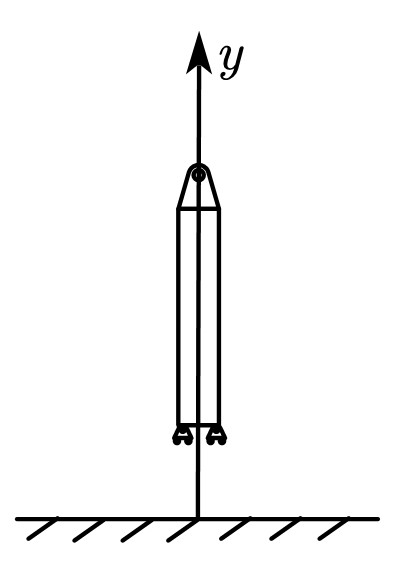
\includegraphics[scale=1.5]{img/graph1.jpg}
        \caption{火箭上升示意图}
        \label{f:1}
    \end{figure}
    设火箭初始质量为$m_0$，其质量按规律$f$衰减，那么
    \[
        m=m_0f\left( t \right) 
    \]
    火箭上升过程中的势能为
    \[
        V=-mgy
    \]  
    动能为
    \[
        T=\frac{1}{2}m\dot{y}^2
    \]
    那么其拉格朗日量为
    \[
        L=\frac{1}{2}m_0f\left( t \right) \dot{y}^2+m_0f\left( t \right) gy
    \]
    将上式代入\eqref{eq:19}式有
    \begin{equation}
        f\left( t \right) \ddot{y}+f\left( t \right) g+v_rf\prime \left( t \right) =0
        \label{eq:3.5}
    \end{equation}
    还可以得到
    \begin{equation}
        \ddot{y}\left( t \right) =-v_r\frac{f\prime \left( t \right)}{f\left( t \right)}-g
        \label{eq:3.6}
    \end{equation}
    若火箭在上升过程中质量按线性规律衰减，衰减系数为$\alpha $，即$f\left( t \right) =1-\alpha t$，那么
    \[
        \left( 1-\alpha t \right) \frac{d^2y}{dt^2}+\left( 1-\alpha t \right) g-v_r\alpha =0
    \]
    上述方程对时间做一次积分有
    \[
        \begin{split}
                \frac{dy}{dt}&=\int{\left( \frac{\alpha v_r}{1-\alpha t}-g \right) dt}+C_1
                \\
                &=-gt-v_r\ln \left( 1-\alpha t \right) +C_1
        \end{split}
    \]
    考虑到$\frac{dy}{dt}|_{t=0}=v_0$，将其代入上式解得$C_1=v_0$，即火箭在上升过程中，其速度随时间的变化关系为
    \[
        \dot{y}\left( t \right) =v_0-gt-v_r\ln \left( 1-\alpha t \right) 
    \]
    取 $v_0 = 2.3\,\mathrm{km}/\mathrm{s}$，$v_r$ 分别为 $3\,\mathrm{km}/\mathrm{s}$、$4\,\mathrm{km}/\mathrm{s}$、$5\,\mathrm{km}/\mathrm{s}$，$\alpha = 0.1/\mathrm{s}$，得到火箭分级后其速度$v\left( \mathrm{km}/\mathrm{s} \right) $随时间$t\left( \mathrm{s} \right) $的变化关系图线，如图\ref{f:2}所示
    \begin{figure}[H]
        \centering
        \label{f:2}
        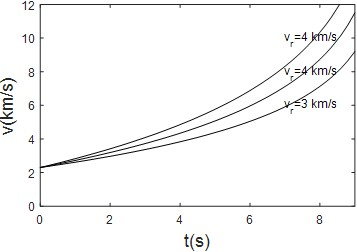
\includegraphics{img/graph2.jpg}
        \caption{不同$v_r$对应的$v$-$t$图线}
    \end{figure}
    可以看到，火箭发生分级后，其速度随时间的变化率会越来越快，速度也越来越快.为求其高度随时间的变化关系，对前式再做一次积分有
    \[
        \begin{split}
            y\left( t \right) &=\int{\left[ v_0-gt-v\ln \left( 1-\alpha t \right) \right]}dt+C_2
            \\
            &=-\frac{1}{2}gt^2
            \\
            &+v_0t+\frac{v_r}{\alpha}\left( 1-\alpha t \right) \left[ \ln \left( 1-\alpha t \right) -1 \right] +C_2
        \end{split}
    \]
    又$y|_{t=0}=y_0$，将其代入上式解得$C_2=y_0-\frac{v_r}{\alpha}$，最终得到火箭分级后其位移随时间的变化关系
    \[
        \begin{split}
            y\left( t \right) &=y_0+\left( v_0+v_r \right) t-\frac{1}{2}gt^2
            \\
            &+\frac{v_r}{\alpha}\left( 1-\alpha t \right) \ln \left( 1-\alpha t \right)
        \end{split} 
    \]
    取$y_0=70\mathrm{km}$，其他数据与绘制图\ref{f:2}时所采取的数据相同，得到其位移随时间的变化关系，如图\ref{f:3}所示
    \begin{figure}[H]
        \centering
        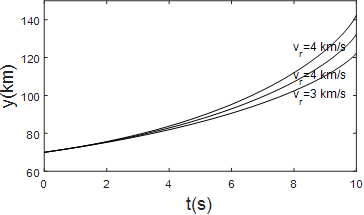
\includegraphics{img/graph3.jpg}
        \caption{不同$v_r$对应的$y$-$t$图线}
        \label{f:3}
    \end{figure}
    若火箭在上升过程中质量按指数规律衰减，衰减系数为$\alpha $，即$f\left( t \right) =e^{-\alpha t}$，那么
    \[
        \ddot{y}+g-v_r\alpha =0
    \]  
    代入相同的初始条件$\frac{dy}{dt}|_{t=0}=v_0$，$y|_{t=0}=y_0$可求得火箭的速度$\dot{y}$和位移$y$随时间的表达式
    \[
        \dot{y}=\left( v_r\alpha -g \right) t+v_0
    \]
    \[
        y=y_0+\frac{1}{2}\left( v_r\alpha -g \right) t^2+v_0t
    \]

    可以发现，当火箭质量按指数规律衰减时，火箭做匀变速直线运动.在不考虑非保守力时，无论火箭质量按何种规律变化，其运动学方程均满足\eqref{eq:3.5}.由\eqref{eq:3.6}还能发现火箭的速度增益取决于其喷出燃料相对火箭的速度  $v_r$以及 $\frac{f\prime}{f}$，当$-v_r\frac{f\prime}{f}>g$时火箭才可正常起飞，$-v_r\frac{f\prime}{f}$ 愈大，其速度增益也愈大.若考虑非保守力，如空气阻力时，应使用更一般的变质量拉格朗日方程，即\eqref{eq:11}，此时会多出阻力广义力，\eqref{eq:3.5}的结构也会因此发生变化.
    \subsection{$\varPhi _{\alpha q}\ne 0$，$\varPhi _{\alpha t}=0$，$\varPhi _{\alpha V}=0$}
    水平桌面上，质量为$M$的小球连接着一条质量线密度为 $\lambda $的匀质细重绳，某时刻，小球突然以初速度 $v_0$竖直向上运动，所受到的阻力与其速度的二次方成正比，比例系数为 $\eta $，欲求其速度随高度变化的函数.
    考虑到小球所受的力有非保守力，故采用\eqref{eq:11}处理此问题.以小球的初始位置为原点，竖直向上为正方向，建立一维坐标系，小球的自由度数为1，故可选取其位置坐标 $y$为其广义坐标.那么小球与在空中的细绳总质量为
    \[
        m\left( y \right) =M+\lambda y
    \]
    其动能为
    \[
        T=\frac{1}{2}m\left( y \right) \dot{y}^2
    \]
    广义力为
    \[
        Q_{\alpha}=-m\left( y \right) g-\eta \dot{y}^2
    \]
    附加广义力的坐标分量为
    \[
        \varPhi _{\alpha q}=-\frac{1}{2}\lambda \dot{y}^2
    \]
    将上述方程代入\eqref{eq:11}有
    \[
        \left( M+\lambda y \right) \ddot{y}+\left( \lambda +\eta \right) \dot{y}^2+\left( M+\lambda y \right) g=0
    \]
    欲解上述方程，令$p=\frac{dy}{dt}$，那么$\frac{d^2y}{dt^2}=\frac{dp}{dy}\frac{dy}{dt}=p\frac{dp}{dy}$那么上式变为
    \[
        p\frac{dp}{dy}+\frac{\lambda +\eta}{M+\lambda y}p^2+g=0
    \]
    令$u=p^2$，那么$\frac{du}{dy}=2p\frac{dp}{dy}$，则
    \[
        \frac{du}{dy}+\frac{2\left( \lambda +\eta \right)}{M+\lambda y}u+2g=0
    \]
    下面采用积分因子法求解上述方程，计算得，方程对应的积分因子为
    \[
        \mu \left( y \right) =\left( M+\lambda y \right) ^{\frac{2\left( \lambda +\eta \right)}{\lambda}}
    \]
    最后得到方程的通解
    \[
        u\left( y \right) =-\frac{2g\left( M+\lambda y \right)}{3\lambda +2\eta}+C\left( M+\lambda y \right) ^{-\frac{2\left( \lambda +\eta \right)}{\lambda}}
    \]
    代入初始条件，$\dot{y}|_{t=0}=v_0$，$y|_{t=0}=0$解得
    \[
        C=\left( v_{0}^{2}+\frac{2Mg}{3\lambda +2\eta} \right) M^{\frac{2\left( \lambda +\eta \right)}{\lambda}}
    \]
    最终得到小球速度随高度的变化的函数
    \[
        \begin{split}
            v^2\left( y \right) &=\left( v_{0}^{2}+\frac{2Mg}{3\lambda +2\eta} \right) \left( \frac{M}{M+\lambda y} \right) ^{\frac{2\left( \lambda +\eta \right)}{\lambda}}
            \\
            &-\frac{2\left( M+\lambda y \right) g}{3\lambda +2\eta}
        \end{split}
    \]
    可以证明，小球高度随时间变化的函数关系不存在显式表达式，但其隐式解可用如下积分表达
    \[
        t=\int_0^y{\frac{dy\prime}{\sqrt{v\left( y\prime \right)}}}
    \]
    \section{牛顿第二定律在狭义相对论情形下的修正}
    由狭义相对论我们知道，质点的质量不再是常数，而是速度的函数，即
    \begin{equation}
        m\left( v \right) =\frac{m_0}{\sqrt{1-\frac{v^2}{c^2}}}
        \label{eq:5.1}
    \end{equation}
    上式中，$m_0$ 为质点的静止质量， $v$为质点运动的速度，$c$ 是光速，在低速情形下 $\frac{v^2}{c^2}$是一个高阶小量，此时质点的质量可视为常量.应用变质量的拉格朗日方程，其广义附加力中的坐标分量和时间分量均为0，而速度分量不为0，即$\varPhi _{\alpha q}=0$ ， $\varPhi _{\alpha t}=0$，$\varPhi _{\alpha \dot{q}}\ne 0$ .考虑一维情况下质点的高速运动，建立一维坐标系，选取 作为其广义坐标，将\eqref{eq:5.1}代入\eqref{eq:14}计算广义附加力的速度分量为
    \begin{equation}
        \varPhi _{\alpha \dot{q}}=\frac{3m_0\dot{x}^2\ddot{x}}{2c^2}\left( 1-\frac{\dot{x}^2}{c^2} \right) ^{-\frac{5}{2}}
        \label{eq:5.2}
    \end{equation}
    考虑到狭义相对论情形下质点的动能为
    \begin{equation}
        T=\frac{1}{2}m_0\dot{x}^2\left( 1-\frac{\dot{x}^2}{c^2} \right) ^{-\frac{1}{2}}
        \label{eq:5.3}
    \end{equation}
    计算$\frac{\partial T}{\partial \dot{x}}$有
    \[
        \frac{\partial T}{\partial \dot{x}}=m_0\dot{x}\left( 1-\frac{\dot{x}^2}{c^2} \right) ^{-\frac{1}{2}}+\frac{1}{2}m_0\frac{\dot{x}^3}{c^2}\left( 1-\frac{\dot{x}^2}{c^2} \right) ^{-\frac{3}{2}}
    \]  
    那么
    \[
        \begin{split}
            \frac{d}{dt}\left( \frac{\partial T}{\partial \dot{x}} \right) &=m_0\ddot{x}\left( 1-\frac{\dot{x}^2}{c^2} \right) ^{-\frac{1}{2}}
            \\
            &+m_0\frac{\dot{x}^2}{c^2}\ddot{x}\left( 1-\frac{\dot{x}^2}{c^2} \right) ^{-\frac{3}{2}}
            \\
            &+\frac{3}{2}m_0\frac{\dot{x}^2}{c^2}\ddot{x}\left( 1-\frac{\dot{x}^2}{c^2} \right) ^{-\frac{3}{2}}
            \\
            &+\frac{3}{2}m_0\frac{\dot{x}^3}{c^4}\ddot{x}\left( 1-\frac{\dot{x}^2}{c^2} \right) ^{-\frac{5}{2}}
            \\
            &=m_0\ddot{x}\left( 1-\frac{\dot{x}^2}{c^2} \right) ^{-\frac{3}{2}}
            \\
            &+\frac{3m_0\dot{x}^2\ddot{x}}{2c^2}\left( 1-\frac{\dot{x}^2}{c^2} \right) ^{-\frac{5}{2}}
        \end{split}
    \]  
    又$\frac{\partial T}{\partial x}=0$，最终由\eqref{eq:11}式可以得到
    \begin{equation}
        Q_{\alpha}=m_0\ddot{x}\gamma ^3
        \label{eq:5.4}
    \end{equation}
    其中$\gamma =\left( 1-\frac{\dot{x}^2}{c^2} \right) ^{-\frac{1}{2}}$，$Q_{\alpha}$为质点受到的广义力，我们令$F=Q_{\alpha}$，那么在狭义相对论下的牛顿第二定律可表达为
    \begin{equation}
        \vec{F}=m_0\ddot{\vec{x}}\gamma ^3
        \label{eq:5.5}
    \end{equation}
    现计算$\frac{d\left( m_0\gamma \dot{x} \right)}{dt}$
    \[
    \begin{split}
        \frac{d\left( m_0\gamma \dot{\vec{x}} \right)}{dt}&=m_0\gamma \ddot{\vec{x}}+\frac{\dot{\vec{x}}^2\ddot{\vec{x}}}{c^2}\gamma ^3
        \\
        &=m_0\ddot{\vec{x}}\gamma \left( 1+\frac{\dot{\vec{x}}^2}{c^2}\gamma ^2 \right) 
        \\
        &=m_0\ddot{\vec{x}}\gamma ^3
    \end{split}
    \]
    即
    \begin{equation}
        F=\frac{d\left( m_0\dot{\vec{x}}\gamma \right)}{dt}
        \label{eq:5.6}
    \end{equation}
    式中$m_0\dot{\vec{x}}\gamma $ 为质点的动量，可见，牛顿第二定律的动量形式在相对论情形下仍然适用.

    \section{总结与展望}
    本文以动量定理为出发点，推导出包含质量导数项的达朗贝尔-拉格朗日原理，与虚功原理相结合，建立了适用于变质量系统的拉格朗日方程。针对保守力系统特有的性质，进一步推导出保守系统下的变质量拉格朗日方程形式。此外，本文将变质量系统划分为四大基本类型：质量显含时间的系统，对应附加广义力的时间分量；质量依赖广义坐标的系统，对应附加广义力的坐标分量； 质量关联广义速度的系统，对应附加广义力的速度分量；前述三类情形的复合系统，对应各分量的综合作用。在经典力学框架下，运用变质量拉格朗日方程，成功求解了多级火箭推进动力学和球绳耦合系统运动学问题；在相对论情形中，通过引入相对论性修正，推导出狭义相对论框架下的变质量动力学方程，完善了相对论情形下的牛顿第二定律表述。值得注意的是，由于能量分析方法在复杂系统研究中具有显著优势，变质量拉格朗日方程在处理多自由度、强耦合的变质量问题时展现出独特的理论价值。但需要指出的是，本文研究仍存在以下局限性：所讨论的案例相对理想化，未涉及非保守力场下的复杂情形；对于相对论性变质量系统的讨论深度有待拓展；应用实例的数量和多样性仍需补充。

    \bibliographystyle{plain}
    \bibliography{Reference}

\end{multicols}

\newpage

\begin{center}
    \heiti\zihao{1}
    Lagrange Equation for Variable Mass and Related Applications
\end{center}

\begin{center}
    Peng Yu

    \textit{(School of Physical Science and Technology, Southwest University,Class of 2023,Physics Class 1)}
\end{center}

\begin{flushleft}                   %文本左对齐（用于取消自动首行缩进）
    \justifying                     %两端对齐
    \textbf{Abstract:}The Lagrange equation plays a crucial role in analytical mechanics, providing a convenient and efficient approach to deriving the differential equations of motion for complex systems from an energy perspective. However, when formulating the Lagrange equation for a system, it is required that the system under study has a constant mass. Therefore, when applying the Lagrange equation to address the dynamic problems of variable mass systems, it is necessary to extend it by incorporating an additional generalized force arising from the mass variation. This paper presents a detailed derivation of the Lagrange equation for variable mass systems using mathematical analysis based on Newton's second law and the principle of virtual work. Furthermore, the derived Lagrange equation for variable mass is applied to study variable mass problems in both classical mechanics and special relativity.\\
    \textbf{Keywords: }variable mass; Lagrange equation; additional generalized force; special relativity
\end{flushleft}

\end{document}